\documentclass[a4paper,american]{llncs}

\usepackage{microtype}%if unwanted, comment out or use option "draft"
\usepackage{amssymb,amsmath}
\usepackage{algorithm,algorithmic}
\usepackage[shortlabels]{enumitem}
\usepackage[nocompress]{cite}
%\usepackage{dsfont}
%\usepackage[american]{babel}
\usepackage{pgf}
\usepackage{tikz}
\usetikzlibrary{shapes.geometric, arrows}
%\usepackage{wrapfig}
%\usepackage{extarrows}
%\usepackage{array}
\usepackage{booktabs}
\usepackage{multicol}
\usepackage{adjustbox}
\usepackage{longtable}
\usepackage{minted}
%\usepackage{matlab-prettifier}
%\usepackage{caption}
% \captionsetup{compatibility=false}
\usepackage{subcaption}
%\usetikzlibrary{arrows,shapes,decorations}
\usepackage{wrapfig}
\usepackage{hyperref}
%\graphicspath{{./graphics/}}%helpful if your graphic files are in another directory

\newcommand{\ToolName}{CLUE~}
\newcommand{\RepoURL}{URL~}

\newif\ifshowcomments
\showcommentstrue % uncomment to show the comments


\definecolor{orange}{RGB}{255,127,0}
\newcommand{\coma}[1]{\ifshowcomments{\color{orange}[AV: #1]}\fi}
\newcommand{\comm}[1]{\ifshowcomments{\color{red}[MT: #1]}\fi}
\newcommand{\comax}[1]{\ifshowcomments{\color{purple} Max: #1}\fi}
\newcommand{\comant}[1]{\ifshowcomments{\color{cyan} {\em [Antonio: #1]}}\fi}
\newcommand{\comalex}[1]{{\color{olive} #1}}
\newcommand*{\myalign}[2]{\multicolumn{1}{#1}{#2}}
%\renewcommand{\coma}[1]{}\cite{DBLP:journals/pnas/CardelliTTV17}
%\renewcommand{\com}[1]{}
%\renewcommand{\comax}[1]{}
\setlength{\tabcolsep}{8pt}
\newcommand{\webpage}{{\color{blue}https://sysma.imtlucca.it/tools/erode/UCTMC/}-\coma{I HAVE TO UPDATE THE ZENODO PAGE}}

\usepackage{array}
\newcolumntype{H}{>{\setbox0=\hbox\bgroup}c<{\egroup}@{}}

\synctex=1

\newcommand{\qedInProof}{
	{\qed}
	%
	%    \IfEqCase{\concurORQuanticolTR}{%
	%        {concur}{{\qed}}%
	%        % you can add more cases here as desired
	%    }%[\PackageError{tree}{Undefined option to tree: #1}{}]%You can decide to launch an exception if cases do not match
}%

\DeclareMathOperator{\sgn}{sgn}

\newcommand{\act}[1]{\xlongrightarrow{#1}}          % transition of with action type [1]

\newcommand{\norm}[1]{\lVert #1 \rVert_2}
\newcommand{\norme}[1]{\lVert #1 \rVert_2}
\newcommand{\normo}[1]{\lVert #1 \rVert_1}
\newcommand{\dt}[1]{\dot{#1}}
\newcommand{\tha}{\hat{t}}
\newcommand{\hh}{\hat{H}}
\newcommand{\hx}{\hat{x}}
\newcommand{\hr}{\hat{r}}
\newcommand{\tr}{\tilde{r}}
\newcommand{\RE}{\mathbb{R}}
\newcommand{\REz}{\mathbb{R}_{\geq0}}
\newcommand{\dom}{\mathcal{D}}
\newcommand{\im}{\mathcal{R}}

\newcommand{\uA}{{u_{\calK}}}
\newcommand{\uS}{{u_S}}
\newcommand{\uAS}{{\uA,\uS}}

\newcommand{\calC}{\mathcal{C}}
\newcommand{\calE}{\mathcal{E}}
\newcommand{\calF}{\mathcal{F}}
\newcommand{\calH}{\mathcal{H}}
\newcommand{\calG}{\mathcal{G}}
\newcommand{\calI}{\mathcal{I}}
\newcommand{\calJ}{\mathcal{J}}
\newcommand{\calP}{\mathcal{P}}
\newcommand{\calK}{\mathcal{K}}
\newcommand{\calR}{\mathcal{R}}
\newcommand{\calS}{\mathcal{S}}
\newcommand{\calU}{\mathcal{U}}
\newcommand{\calW}{\mathcal{W}}

\newcommand{\tF}{\tilde{F}}

\DeclareMathOperator*{\argmax}{arg\,max}
\DeclareMathOperator*{\rank}{rank}
\DeclareMathOperator*{\rsp}{rowsp}
\DeclareMathOperator{\dev}{dev}


\newcommand{\upa}{\underline{p}}
\newcommand{\upi}{\underline{\pi}}
\newcommand{\upia}{\underline{\pi}^\ast}
\newcommand{\uphi}{\underline{\phi}}
\newcommand{\pia}{\pi^\ast}

\newcommand{\deps}{\Delta \varepsilon}

\newcommand{\fru}{\mathfrak{u}}
\newcommand{\frut}{\mathfrak{\tilde{u}}}


\newcommand{\eps}{\varepsilon}
\newcommand{\epst}{\varepsilon'}
\newcommand{\epsp}{\varepsilon^+}
\newcommand{\epso}{\varepsilon^{\mathit{old}}}
\newcommand{\epsn}{\varepsilon^{\mathit{new}}}
\newcommand{\hk}{\hat{\kappa}}
\newcommand{\frb}{\mathfrak{b}}

%\newcommand{\dt}{\Delta t}
%\newcommand{\dtau}{\Delta \tau}
%\newcommand{\dte}{\Delta t_{\mathit{err}}}
%\newcommand{\dth}{\DeCLUEa}


\renewcommand{\algorithmicrequire}{\textbf{Input:}}
\renewcommand{\algorithmicensure}{\textbf{Output:}}

%\let\example\undefined
%\newtheorem{example}{Example}
%\newtheorem{myExample}[example]{Example}

\newenvironment{myExample}{\begin{example}}{\hfill $\blacksquare$ \end{example}}
\newif\ifshowproofs
\showproofsfalse

\begin{document}



%\title{\ToolName - Lumping of Ordinary Differential Equations}

\institute{
	%University of Oxford, UK
	%\and
	%TU Wien, Austria
	%\and
	Aalborg University, Denmark
	\and
	IMT School for Advanced Studies Lucca, Italy
	\and
	Sant'Anna School of Advanced Studies, Pisa, Italy
	\and
	DTU Technical University of Denmark
}

\author{
Antonio Jim\'{e}nez-Pastor \inst{1} \and
Alexander Leguizamon-Robayo \inst{1} \and
\newline
%Micro Tribastone\inst{2}
Max Tschaikowski \inst{1} \and
Andrea Vandin\inst{3,4}
}


%\author{Luca Cardelli\inst{1} \and Radu Grosu\inst{2} \and Kim G. Larsen\inst{3} \\ Mirco Tribastone\inst{4} \and Max Tschaikowski\inst{3} \and Andrea Vandin\inst{5,6}}


%
%
%\Copyright{L. Cardelli, K. G. Larsen, R. Grosu, M. Tribastone, M. Tschaikowski, and A. Vandin} %mandatory, please use full first names. LIPIcs license is "CC-BY";  http://creativecommons.org/licenses/by/3.0/
%
%\subjclass{D.2.4, G.1.7, J.2}%  Dummy classification -- please refer to \url{http://www.acm.org/about/class/ccs98-html}}% mandatory: Please choose ACM 1998 classifications from http://www.acm.org/about/class/ccs98-html . E.g., cite as "F.1.1 Models of Computation".
%\keywords{Uncertain Markov chains -- Lumpability -- Model Checking}% mandatory: Please provide 1-5 keywords
%% Author macros::end %%%%%%%%%%%%%%%%%%%%%%%%%%%%%%%%%%%%%%%%%%%%%%%%%
%
%%Editor-only macros:: begin (do not touch as author)%%%%%%%%%%%%%%%%%%%%%%%%%%%%%%%%%%
%\serieslogo{}%please provide filename (without suffix)
%\volumeinfo%(easychair interface)
%{Billy Editor and Bill Editors}% editors
%{2}% number of editors: 1, 2, ....
%{Conference title on which this volume is based on}% event
%{1}% volume
%{1}% issue
%{1}% starting page number
%\EventShortName{}
%\DOI{10.4230/LIPIcs.xxx.yyy.p}% to be completed by the volume editor
%% Editor-only macros::end %%%%%%%%%%%%%%%%%%%%%%%%%%%%%%%%%%%%%%%%%%%%%%%
%

% Author macros::begin %%%%%%%%%%%%%%%%%%%%%%%%%%%%%%%%%%%%%%%%%%%%%%%%
\title{Approximate Reductions of \newline Rational Dynamical Systems in CLUE}
%\titlerunning{Approximate Constrained Lumping} %optional, in case that the title is too long; the running title should fit into the top page column


\allowdisplaybreaks[0]

\maketitle

\begin{abstract}
	%!TEX root = 2024-cmsb_tool.tex

In life sciences, deriving insights from dynamical systems can be challenging due to the large number of state variables involved. 
To address this, model reduction techniques can be used to project the system onto a lower-dimensional state space.
CLUE is a tool that computes exact linear reductions for rational systems of ordinary differential equations.
In this paper, we present an extension of CLUE to include approximate reductions which allow for larger aggregating power at the expense of a bounded error.
Additionally, our extension includes new functionalities such as an interface to the model database OdeBase repository and simulation tools for exploratory analyses.


\end{abstract}

\keywords{Approximate reduction $\cdot$ Dynamical systems $\cdot$ Constrained lumping}


\section{Introduction}\label{sec_intro}

%!TEX root = 2024-cmsb_tool.tex
%\comm{we need to cite some work by PC members (i.e., Tanja etc), maybe from our first CONCUR paper, QEST'18 Lumping the Approximate Master Equation for Multistate Processes on Complex Networks.}
Dynamical models of biochemical systems help discover mechanistic principles in living organisms and predict their behavior under unseen circumstances.
Realistic and accurate models, however, often require considerable detail that inevitably leads to large state spaces.
This hinders both human intelligibility and numerical/computational analysis.
For example, even the relatively primary mechanism of protein phosphorylation yields, in the worst case, a combinatorial state space as a function of the number of phosphorylation sites~\cite{FEBS:FEBS7027}.

As a general way to cope with large state spaces, model reduction aims at providing a lower-dimensional representation of the system under study that retains some dynamical properties of interest to the modeler.
In applications to systems biology, it is beneficial that the reduced state space keeps physical interpretability, mainly when the model is used to validate mechanistic hypotheses~\cite{10.1093/bioinformatics/btn035,21899762,Apri201216}.
There is a variety of approaches in this context, such as those exploiting time-scale separation properties~\cite{okino1998,DBLP:journals/tac/WhitbyCKLTT22}, quasi-steady-state approximation~\cite{SegelS89,radulescu2012reduction}, heuristic fitness functions~\cite{10.1145/3071178.3071265}, spatial regularity~\cite{DBLP:journals/pe/TschaikowskiT17}, sensitivity analysis~\cite{Snowden:2017aa} and, at last, conservation analysis, which detects linear combinations of variables that are constant at all times~\cite{10.1093/bioinformatics/bti800}.

By lumping, one generally refers to the latter class, with a self-consistent system of dynamical equations comprised of a set of macro-variables, each given in terms of combination of the original ones~\cite{okino1998,Snowden:2017aa,DBLP:conf/qest/GrossmannKBW18,backenkohler2021abstraction,DBLP:journals/pe/AbateACK21}.
In linear lumping, this reduction is expressed as a linear transformation of the original state variables.
Since this can destroy physical intelligibility in general, \emph{constrained lumping} allows restricting to only part of the state by defining linear combinations of state variables that ought to be preserved in the reduction~\cite{LI199195}.
Lumping techniques of Markov chains date back to the early nineties~\cite{Larsen19911}.
These were later extended to stochastic process algebra~\cite{10.1007/978-0-387-09680-3_18,10.1007/978-3-540-88479-8_13,10.1093/comjnl/bxr094,DBLP:conf/splc/Tribastone14,TSCHAIKOWSKI2014140}, and have been expanded more recently to efficient algorithmic approaches for stochastic chemical reaction networks~\cite{DBLP:journals/bioinformatics/CardelliPTTVW21} and deterministic models of biological systems~\cite{CARDELLI2019132,pnas17,DBLP:conf/lics/CardelliTTV16}.
In these works, reduction mappings are linear mappings induced by a partition (i.e., an equivalence relation) of state variables; in the aggregated system each macro-variable represents the sum of the original variables of a partition block.

In this paper we are concerned with systems of ordinary differential equations (ODEs) with analytical derivatives.
\comalex{
	As concrete instances, we mention systems with \textit{rational} and \textit{polynomial} derivatives which cover kinetic models with Hill~\cite{voit_biochemical_2013}, Michaelis-Menten~\cite{voit_biochemical_2013} and mass-action semantics (e.g.,~\cite{Voit:2013aa,DBLP:journals/biosystems/TrojakSPB23});
	and that are also rich enough to model electric circuits~\cite{DBLP:journals/nc/CardelliTT20}.
	%kinetic models developed via  and  which 
	%These show up in practice as systems with \textit{polynomial} derivatives when the denominator is 1.
	%these systems show up in two ways, \textit{polynomial} (e.g.,  when the denominator is 1\coma{do we really need this example?}) and  systems.
	For polynomial systems, CLUE has been presented as an algorithm that efficiently computes constrained linear lumpings~\cite{ovchinnikov_clue_2021}.
	While previous work required the symbolic computation of the eigenvalues of a nonconstant matrix~\cite{LiRabitz,LI199195}, CLUE avoids these computational shortcomings, thus enabling the analysis of models with several thousands of equations on standard hardware.
}
%CLUE avoids the computational shortcomings of previous work due to the symbolic computation of the eigenvalues of a nonconstant matrix~\cite{LiRabitz,LI199195}, thus enabling the analysis of models with several thousands of equations on standard hardware.
In particular, CLUE can compute \emph{the smallest} linear dimensional reduction that preserves the dynamics of arbitrary linear combinations of original state variables given by the user.
While it is possible to extend CLUE to rational systems~\cite{jimenez_clue_2022} by means of symbolic computations, this approach quickly becomes computationally expensive.
This problem can be avoided by efficiently creating a representation of the dynamics by sampling it at different points using automatic differentiation~\cite{jimenez_clue_2022}.

The aforementioned lumping approaches are \emph{exact}, in that the reduced model does not incur any approximation error (but only loss of information because, in general, the aggregation map is not invertible).
Approximate lumping is a natural extension that has been studied for a long time (e.g.,~\cite{LI1990977}).
Indeed, although exact reduction methods have been experimentally proved successful in a large variety of biological systems (e.g.,~\cite{SBML}), approximate reductions can be more robust to parametric uncertainty---which notoriously affects systems biology models (e.g.,~\cite{doi:10.1098/rsif.2017.0237,DBLP:conf/cmsb/BarnatBBDHPS17})---and offer a flexible trade-off between the aggressiveness of the reduction and its precision.
For partition-based lumping algorithms, this has been recently explored.
In~\cite{DBLP:conf/qest/CardelliTTV18}, the authors present an algorithm for approximate aggregation parameterized by a tolerance $\varepsilon$, which, informally, relaxes an underlying criterion of equality for two variables to be exactly lumped into the same block.
Similarly, for linear lumpings, an approximate extension to CLUE for polynomial systems has been presented in~\cite{leguizamon-robayo_approximate_2023}.
This approach relaxes the conditions for exact lumping using a \emph{lumping tolerance} parameter that is roughly related to how close a lumping matrix is to an exact lumping.
In particular, the authors show that the actual error is proportional to the lumping tolerance.

\comalex{
	In this paper, we extend approximate constrained lumping~\cite{leguizamon-robayo_approximate_2023} to systems of ODEs with general analytical drifts including rational drifts, while still working in polynomial time.
	Using a prototype implementation, we evaluate our approach on five polynomial models and four rational models representative of the literature.
	We also propose a new way to compute an approximate lumping tolerance based on the expected size of the reduced model.
	Overall, the numerical results recover previous ones~\cite{leguizamon-robayo_approximate_2023} and show that our extension can lead to substantially smaller reduced models while introducing limited errors in the dynamics both for polynomial and rational systems.
	In light of these results, we propose a heuristic that provides one with a value to determine a lumping tolerance that outputs a reduction with an acceptable error.
}
\coma{Isn't this just a repetition of 'We also propose a new way to compute \ldots'??}


\paragraph{\textbf{Further related work.}} We are complementary to classic works~\cite{LI1990977,LI199195} which do not address the efficient algorithmic computation of lumping. Moreover, we are more general than~\cite{iacobelli_lumpability_2013,tac15,DBLP:conf/qest/CardelliTTV18} which consider so-called ``proper'' lumping (i.e.,~\cite{Snowden:2017aa}) where each state variable appears in exactly one aggregated variable. %The algorithm takes as input a numerical tolerance and computes an approximate constrained lumping whose error is guaranteed to be proportional to the lumping tolerance. %The estimation rests upon Gronwall's inequality that has been used in~\cite{}.
Likewise, we are complementary to rule-based reduction techniques~\cite{Feret21042009} which are independent of kinetic parameters~\cite{concur15}. As less closely related abstraction techniques, we mention (bisimulation) distance approaches for the approximate reduction of Markov chains~\cite{DBLP:conf/tacas/BacciBLM13,DBLP:conf/concur/DacaHKP16} and proper orthogonal projection~\cite{antoulas}, which, however, apply to linear systems. Abstraction of chemical reaction networks by means of learning~\cite{DBLP:journals/iandc/RepinP21,DBLP:conf/cmsb/CairoliCB21} and simulation~\cite{DBLP:conf/cmsb/HelfrichCKM22} are complementary to lumping methods.


\paragraph{\textbf{Outline.}} Section~\ref{sec_pre} provides necessary preliminary notions, Section~\ref{sec_theory} introduces approximate constrained lumping, while Section~\ref{sec:computing} discusses how to compute it and how to choose the lumping tolerance value. Section~\ref{sec_eval} evaluates our proposal on models from the literature, while Section~\ref{sec_conc} concludes the paper.



\paragraph{\textbf{Notation.}}
\comalex{
For a function $f$, we denote its domain by $\dom(f)$.
The derivative with respect to time of a function $x : [0,T] \to \RE^m$ is denoted by $\dot{x}$.
We denote a dynamical system by $\dot{x} = f(x)$, and denote its initial condition by $x(0)=x^{0}$.
For $f: \mathbb{R}^{m} \to \mathbb{R}^{n}$,  we denote the Jacobian of $f$ at $x$ by $J(x)$.
%For any vector $x \in \mathbb{R}^{m}$, we denote by $\mathbb{R}[x]$ and  $\mathbb{R}(x)$ the rings of polynomial functions and rational functions of $x$ with real coefficients respectively.
Given a matrix $L \in \mathbb{R}^{m\times n} $, the rowspace of $L$ or the vector space generated by the rows of $L$ is denoted by $\rsp(L)$.
We denote by $\bar{L} \in \mathbb{R}^{n \times m}$ a  pseudoinverse of $L$ (i.e. $L\bar{L}= I_{n}$ where $I_{n} \in \mathbb{R}^{n\times n}$ is the identity matrix).
We reserve the term \textit{rational} for models with a non-trivial denominator on their right-hand side.
}
%The term \textit{pseudoinverse} refers to a right pseudoinverse.
\coma{what do we mean? We already write explicitly 'a right pseudoinverse' in the previous sentence. Either we remove this sentence, or we remove right from the previous sentence}







\section{Preliminaries}\label{sec_pre}

%!TEX root = 2024-cmsb_tool.tex
%Introduce what lumping is in the case of a rational system. 
Constrained lumping is a reduction method that allows to reduce a system in a way that it preserves a linear combination of variables of interest.
Suppose we are interested in the evolution of an observable $x_1$ and its evolution is described by the following system of ODEs
\begin{equation} \label{eq:example1}
	\dot{x_{1}} = \frac {x_{2}^{2} +4x_{2}x_{3} +4x_{3}^{2}}{x_{1}^{2} + 1 },\qquad
	\dot{x_{2}} = \frac{2x_{1}-4x_{3}}{x_{2}+2x_{3} + 1},\qquad
	\dot{x_{3}} = \frac{-x_{1}-x_{2}}{x_{2}+2x_{3}+1}.
\end{equation}
The matrix $L = (1 \ 0\ 0, 0\ 1\  2)^{T}$ is an \textit{exact constrained lumping} of dimension 2, since it allows one to construct a smaller self-consistent system in terms of the \textit{macro-variables} $y_1= x_1$ and $ y_2 = x_2 + 2x_3$, as follows:
\begin{equation*}
	\begin{pmatrix}
		\dot{y}_{1} \\
		\dot{y}_{2}
	\end{pmatrix}
	=
	\begin{pmatrix}
		\dot{x}_{1} \\
		\dot{x}_{2} +2 \dot{x}_{3}
	\end{pmatrix}
	=
	\begin{pmatrix}
		\frac{(x_{2}+2x_{3})^{2}}{x_{1}^{2}+1} \\
		\frac{-2x_{2}-4x_{3}}{x_{2}+2x_{3}}
	\end{pmatrix}
	=
	\begin{pmatrix}
		\frac{y_{2}^{2}}{y_{1}^{2}+1} \\
		\frac{-2y_{2}}{y_{2}+1}
	\end{pmatrix}.
\end{equation*}
The matrix $L$ is a \textit{constrained} lumping since the evolution of $x_1$ can be directly recovered from the evolution of $y_1$.
It is \textit{exact} as there the evolution of $x_1$ can be recovered without any errors by using the lower dimensional system.
In general, given a system of ODEs $\dot{x} = f(x)$  and an exact lumping $L$ a self-consistent reduced system can be constructed as
$y= L f(\bar{L}x)$, where $y = Lx$, and $\bar{L}$ is a right-pseudo inverse of $L$.
In this case, $\bar{L} = (1 \ 0, 0 \ 0.2, 0 \ 0.4)^{T}$.

Now, suppose the evolution of $x_1$ is described by a slightly different system:
\begin{equation} \label{eq:examplepert}
	\dot{x}_{1} = \frac {x_{2}^{2} +4.05x_{2}x_{3} +4x_{3}^{2}}{x_{1}^{2} + 1 },~
	\dot{x}_{2} = \frac{2x_{1}-4x_{3}}{x_{2}+2x_{3} + 1},~
	\dot{x}_{3} = \frac{-x_{1}-x_{2}}{x_{2}+2x_{3}+1}.
\end{equation}
In this case, it is not possible to construct an exact approximate constrained lumping.
However, by relaxing the conditions for lumping the matrix $L = (1 \ 0\ 0, 0\ 1\  2)^{T}$ we can compute a smaller system that preserves $x_1$ up to an error, as follows.
\begin{equation*}
	\begin{pmatrix}
		\dot{y}_{1} \\
		\dot{y}_{2}
	\end{pmatrix}
	= L f \left(  \bar{L}        \begin{pmatrix}
		y_{1} \\
		y_{2}
	\end{pmatrix}
	\right)
	=
	L f \left(
	\begin{pmatrix}
			y_{1} & 0        \\
			0     & 0.2y_{2} \\
			0     & 0.4y_{2}
		\end{pmatrix} \right)
	=
	%L \begin{pmatrix}
	%1.004y_{2}^{2}    \\
	%2y_{1} - 1.6y_{2} \\
	%-y_{1}-0.2y_{2}
	%\end{pmatrix}=
	\begin{pmatrix}
		\frac{1.004y_{2}^{2}}{y_{1}^{2}+1} \\
		\frac{-2y_{2}}{y_{2}+1}
	\end{pmatrix}.
\end{equation*}
\begin{wrapfigure}[12]{r}{0.4\textwidth}
	\centering
	\vspace{-0.5cm}
	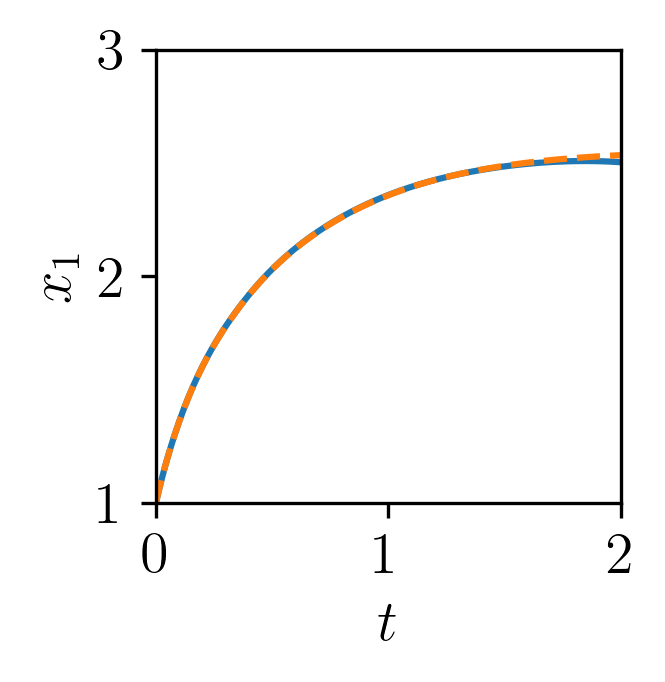
\includegraphics[width=0.7\linewidth]{./img/sim_red_example.png}
	\caption{Evolution of the reduced (orange) and original (blue).}
	\label{fig:apperr:sim}
\end{wrapfigure}
This means that the evolution of $x_1$ will be recovered up to an error.
Figure~\ref{fig:apperr:sim} shows the evolution of $x_1$ computed via the original and reduced system for initial conditions $x = (1,0,0)^{T}$.
Note that by using an approximate reduction it is possible to reduce a system that was not exactly reducible while still obtaining a simulation with low error.
The detailed theory of approximate constrained lumping for polynomial systems, including the algorithm to compute them and how to bound the introduced errors, can be found in~\cite{leguizamon-robayo_approximate_2023}.



%In general, for an ODE system $\dot{x}= f(x)$  
%Consider a system of ODEs $\dot{x}= f(x)$, where $f: \mathbb{R}^{n}\to \mathbb{R}^{n}$ and each entry of $f$ is a rational function. 
%We say that a linear transformation $L: \mathbb{R}^{n}\to \mathbb{R}^{m}$ with $m< n$ is an \textit{exact lumping} if there exists a function $g:\mathbb{R}^{m} \to \mathbb{R}^{m}$, such that $L\circ f = g \circ L$. 
%For an initial condition $x(0) \in \mathbb{R}^n$ and an exact lumping $L$, there is a corresponding initial condition $y(0)$ in the lumped variables given by $y(0) = L x(0)$.
%A self-consistent system of ODEs can be constructed as follows \[L\dot{x} = Lf(x)= g(Lx)=g(y)=\dot{y}\ .\]



%Assume now that the dynamics are given by 
%\begin{equation} \label{eq:examplepert}
%\dot{x}_{1} = \frac {x_{2}^{2} +4.05x_{2}x_{3} +4x_{3}^{2}}{x_{1}^{2} + 1 },~
%\dot{x}_{2} = \frac{2x_{1}-4x_{3}}{x_{2}+2x_{3} + 1},~
%\dot{x}_{3} = \frac{-x_{1}-x_{2}}{x_{2}+2x_{3}+1}.
%\end{equation}
%We still want to preserve the observable $x_1$. 
%In this case, the matrix $L = (1 \ 0\ 0, 0\ 1\  2)^{T}$ is not 



%In this paper, we study systems of ODEs with analytic derivatives of the form:
%\begin{equation}
%\dot{x}  = f(x), \label{eq:ode}
%\end{equation}
%where $f: \mathbb{R}^{m} \to \mathbb{R}^{m}, x\mapsto (f_{1}(x), \dots, f_{m}(x))^{T}$ and $f_{i}$ is an analytic function,  for $i=1,\dots, m$.

%\begin{definition}\label{def:lump}
%Given a system of ODEs of the form given by Equation~\eqref{eq:ode}, and a full rank matrix $L\in \mathbb{R}^{l\times m}$ with $l< m$,
%we say that $L$ is an \emph{exact lumping of dimension $l$} (or that the system is \emph{exactly lumpable} by $L$) if there exists a function $g: \mathbb{R}^{l} \to \mathbb{R}^{l}$ with polynomial entries such that $Lf = g\circ L$.
%\end{definition}


%\begin{definition}\label{def:constlump}
%Given a system of ODEs of the form given by Equation~\eqref{eq:ode}, and an exact lumping $L\in \mathbb{R}^{l\times m}$, we say that $y= Lx$ are the \emph{reduced (or lumped) variables}, 	and their evolution is given by the \emph{reduced system} $ \dot{y}= g(y)$.
%\end{definition}

%Given an initial condition $x^{0} \in \mathbb{R}^n$ and an exact lumping $L$, there is a corresponding initial condition $y^{0}$ in the lumped variables given by $y^{0} = L x^{0}$.
%Similarly, since $y=Lx$ and $g\circ L = Lf$, we have that \[L\dot{x} = Lf(x)= g(Lx)=g(y)=\dot{y}\ .\]
%This means that we can study the evolution of the lumped variables $y(t)$ by solving the (smaller) reduced system rather than the (larger) original one.

%Suppose that we want now to recover the evolution of some linear combination of state variables.
%To answer whether this is possible, we introduce the notion of constrained lumping.

%\begin{definition}
%Let $x_{obs}= Mx$ for some matrix $M \in \mathbb{R}^{p\times m}$, for $p< m$.
%We say that a lumping $L$  is a \emph{constrained lumping} with \emph{observables} $x_{obs}$ if  $\rsp(M) \subseteq \rsp(L)$.
%This means that each entry of $x_{obs}$ is a linear combination of the reduced 	variables $y$. 	
%\end{definition}

%\begin{myExample}
%Suppose we are interested in observing the quantity $2x_{1}+x_{2}+2x_{3}$ where the evolution is given by the system~\eqref{eq:example1}.
%In this case $x_{obs}= Mx$ with $M = ( 2\ 1\ 2)$.
%We can see that  $L$ from Example \ref{ex:firstode} is a constrained lumping as we can recover the observable from the reduced system, i.e., $ x_{obs}=2y_{1}+y_{2}$.
%Suppose now that we want to observe the quantity $x_{1}+x_{2}+x_{3}$.
%In this case $M = ( 1\ 1\ 1)$ and so the matrix $L$ is not a constrained lumping as there is no way to obtain $x_{obs}$ as a linear combination of $y_{1}$ and $y_{2}$.
%\end{myExample}

%To understand how a constrained lumping can be computed, we first review the following known characterization of lumping.

%\begin{theorem}[Characterization of Exact Lumping~\cite{tomlin_effect_1997}]\label{thm:lumping}
%Given a system of $m$ ODEs of the form given by Equation\eqref{eq:ode} and a matrix $L\in \mathbb{R}^{l\times m}$ with rank $l$, the following are equivalent.
%\begin{enumerate}
%\item The system is exactly lumpable by $L$.
%\item\label{thm:lumping:inverse} For any pseudoinverse $\bar{L}$ of $L$, $Lf = (Lf) \circ \bar{L}L$.
%\item\label{thm:lumping:invariant} The row space of $L$ is invariant under $J(x)$ for all $x\in \mathbb{R}^{m}$, where $J(x)$ is the total derivative of $f$ at $x$, known also as the Jacobian.
%More formally, $\rsp(L J(x)) \subseteq \rsp(L)$ for all $x \in \RE^m$.
%\end{enumerate}
%\end{theorem}

%The characterization of exact lumpings in Theorem~\ref{thm:lumping} provides us a way to compute a constrained lumping $L$.
%This is because thanks to Point~\ref{thm:lumping:invariant}, the problem of computing a lumping is equivalent to the problem of finding a $J(x)$-invariant subspace of $\mathbb{R}^{m}$ for all $x \in \mathbb{R}^{m}$.
%However, $J(x)$ is a matrix whose entries are functions of $x$.
%In other words, there is a different real-valued matrix for each $x \in \mathbb{R}^{m}$.
%To circumvent this issue we require the following result:

%\begin{theorem}[{\cite[Lemma 1]{jimenez_clue_2022}}]\label{thm:repJ}
%Consider a system ODEs of the form given by Equation~\eqref{eq:ode} and let $J(x)$ be the Jacobian matrix of $f$.
%Let $\mathcal{B}$ be any set of real-valued matrices spanning the $\mathbb{R}-$vector space $$\mathcal{V}_{J}:=\left< J(x) | x \in \mathbb{R}^{m} \text{ and $J(x)$ is well-defined}\right>.$$
%Then $L$ is a lumping of~\eqref{eq:ode} if and only if $\rsp(L)$ is invariant to each $J_i \in \mathcal{B}$.
%\end{theorem}

%A set of matrices $\{J_1,\dots, J_N\}$ can be found analytically when $J(x)$ can be represented as
%\begin{equation}\label{eq:jacrep}
%J(x) = \sum_{i=0}^{N}J_{i}\mu_{i}(x),
%\end{equation}
%where $\left\{\mu_{i}(x)\ :\ i\in\{0,\ldots,N\}\right\}$ is a set of analytic functions.
%When working with polynomial systems, each of the entries of $J(x)$ is a polynomial and so each $\mu_i$ corresponds to the monomials of $J(x)$.

%\comalex{
%In particular, for rational systems, a  similar representation of $J(x)$ can be obtained symbolically by differentiating $f(x)$ and then multiplying by the minimum common denominator.
%In practice, this approach is computationally unfeasible due to the fact that this symbolic approach results in an explosion of the number of monomials in $J(x)$.
%\coma{sentence difficult to parse. Does it explode after differentiating (i.e. we differentiate after using the mcd? or we apply the mcd after differentiating?}
%To avoid any explicit symbolic computations, a representation $\{J_1,\dots, J_N\}$ can be obtained by sampling $f(x)$ at different points and using automatic differentiation.
%%In this way, we avoid any explicit symbolic computation of the Jacobian matrix.
%The general idea of this sampling procedure is formalized by Algorithm~\ref{alg:findJ}.
%Our implementation followed the recommendations found in~\cite[Section 3.4]{jimenez_clue_2022}.
%These guidelines show how to efficiently sample $J(x)$ to obtain a correct representation of $\mathcal{V}_{J}$ with high probability.

%\begin{algorithm}[h]
%\caption{\footnotesize Representing $J(x)$}\label{alg:findJ}
%%\algsetup{linenosize=\tiny}
%%\scriptsize
%\begin{algorithmic}[1]
%\REQUIRE
%$f: \mathbb{R}^{m} \to \mathbb{R}^{m}$\\
%a compact set $\Omega \subset \mathbb{R}^{m}$\\
%\STATE {\textbf{set} $N=0$}
%\REPEAT
%\STATE {\textbf{set} $N=N+1$}
%\STATE {\textbf{compute} $x_N$ sampling uniformly from $\Omega$ }
%\STATE {\textbf{compute} $J_N=J(x_N)$ using automatic differentiation}
%\UNTIL{$J_N \in \left< J_i | 1\leq i \leq N-1 \right>$}

%\RETURN {$\{J_1,\dots, J_{N-1}\}$}.
%\end{algorithmic}
%\end{algorithm}

%\coma{Before talking about alg 1 we need to introduce it. We shall say: This can be implemented as shown in Algorithm~\ref{alg:findJ}, using the recommendations... }
%%The following example shows Algorithm~\ref{alg:findJ} in action.

%\comalex{
%\begin{myExample}\label{ex:findJ}
%Consider the system given by  Example~\ref{ex:firstode}.
%In this case, we first use the analytic approach to find a basis for $\mathcal{V}_{J}$.
%By symbolically differentiating and multiplying by the minimum common denominator, we infer that the Jacobian of $f(x)$ is of the form $J(x)= B(x)/q(x)$ where the minimum common denominator is
%$ q(x)= (x_{1}^{2} +1)^{2}(x_{2}+2x_{3}+1)^{2}$
%and $B(x)$ is a matrix with polynomial entries up to degree 5.
%Notice that to obtain a representation we need to expand all the terms in $B(x)$.
%%[(5, (1, 5, 2)), (5, (3, 3, 2)), (5, (5, 2, 3)), (5, (2, 4, 3))]
%These symbolic computations can be avoided by using Algorithm~\ref{alg:findJ}.
%Following~\cite{jimenez_clue_2022}, we find that the dimension of $\mathcal{V}_{J}$ is 6.
%The set $\{J_1,\dots,J_6\}$ is obtained by evaluating $J(x)$ at the following points: $
%x_1 = (1, 5, 2),~x_2 = (3, 3, 2),~x_3 = (5, 2, 3),~x_4 = (2, 4, 3),~x_5 = (3, 2, 4),~x_6 = (4, 3, 2).$
%For the sake of brevity, we only display the first 4 matrices $J_i$:
%%[ 0  0  0  2 -2 -8 -1  0  2]
%%[ 0.    2.    4.    1.    0.   -2.   -0.5  -0.25  0.5 ]
%%[ 0.     4.     8.     0.667  0.444 -0.444 -0.333 -0.333  0.   ]
%%[-40.5    9.    18.     0.2    0.06  -0.28  -0.1   -0.04   0.12]
%\begin{equation*}
%\begin{split}
%J_1 &=
%\begin{pmatrix}
%0  & 0  & 0  \\
%2  & -2 & -8 \\
%-1 & 0  & 2
%\end{pmatrix},\\
%J_3 &=
%\begin{pmatrix}
%0      & 4      & 8      \\
%0.667  & 0.444  & -0.444 \\
%-0.333 & -0.333 & 0
%\end{pmatrix},
%\end{split}
%\hspace{1cm}
%\begin{split}
%J_2 &=
%\begin{pmatrix}
%0    & 2     & 4   \\
%1    & 0     & -2  \\
%-0.5 & -0.25 & 0.5
%\end{pmatrix},\\
%J_4 &=
%\begin{pmatrix}
%-40.5  & 9      & 18     \\
%0.200  & 0.060  & -0.280 \\
%-0.100 & -0.040 & 0.120
%\end{pmatrix}.
%\end{split}
%\end{equation*}
%\end{myExample}
%}
%%\coma{The alignment is completely messed up. Can we at least align the '='?}


%We see that Algorithm~\ref{alg:findJ} outputs a set of matrices $\{ J_1,\dots, J_N\}$
%%\coma{$N$ or $M$? the algorithm says $M$} 
%spanning $\mathcal{V}_{J}$.
%Given such a set, Theorem~\ref{thm:repJ} provides an algorithmic way to find a constrained lumping $L$ by performing a finite number of checks over real-valued vectors.
%This is shown in Algorithm~\ref{alg:findL}.
%The use of Algorithms~\ref{alg:findJ} and~\ref{alg:findL} to obtain a constrained lumping $L$ is summarized in Algorithm~\ref{alg:clue}.
%%The aforementioned reasoning gives rise to a computational way to verify Point~\ref{thm:lumping:invariant} in Theorem~\ref{thm:lumping}, i.e.,  Algorithm~\ref{alg:clue}.
%\coma{It is a bit weird that we cite Alg3 before Alg2. Can we rephrase this sentence?}
%%Using Equation~\eqref{eq:jacrep},the condition of Theorem~\ref{thm:repJ} can by checked by noticing that all rows $r$ of $L$, $rJ(x) \in \rsp(L)$ for all $x$ if and only if $rJ_{i} \in \rsp(L)$ for $i=1,\dots, N$.
%%This result leads to Algorithm~\ref{alg:findL}.

%\hspace{-0.65cm}
%\begin{minipage}[t]{0.47\textwidth}
%\begin{algorithm}[H]
%\caption{\footnotesize Computation of $L$}\label{alg:findL}
%\algsetup{linenosize=\tiny}
%\scriptsize
%\begin{algorithmic}[1]
%\REQUIRE
%a set of matrices $\left\{ J_1,\dots,J_N \right\}$ spanning $\mathcal{V}_{J}$ (Theorem \ref{thm:repJ});\\
%a $p \times m$ matrix $M$ with row rank $p$.\label{alg:findL:M}

%\STATE \textbf{set} $L := M$
%\REPEAT
%\FORALL{$1 \leq i \leq \kappa$ and rows $r$ of $L$}
%\STATE {\textbf{compute} $r J_i$ }
%\IF{$rJ_{i}\notin \rsp(L)$} \label{alg:findL:check}
%\STATE {\textbf{append} row $r J_i$ to $L$}\label{alg:findL:append}
%\ENDIF
%\ENDFOR
%\UNTIL{no rows are appended to $L$}

%\RETURN Lumping matrix $L$.
%\end{algorithmic}
%\end{algorithm}
%\vspace{0.01cm}
%\end{minipage}
%\hfill
%\begin{minipage}[t]{0.47\textwidth}
%\begin{algorithm}[H]
%\caption{\footnotesize Constrained lumping \cite{ovchinnikov_clue_2021} }\label{alg:clue}
%\algsetup{linenosize=\tiny}
%\scriptsize
%\begin{algorithmic}[1]
%\REQUIRE \!\!a\! system \!$\dot{x} \!=\!\! f(x)\!$ of $\!m\!$ \! ODEs;\\
%a $p \times m$ matrix $M$ with row rank $p$.\\

%%\STATE \textbf{compute} $J(x)$, the Jacobian 			of $f(x)$

%\STATE \textbf{compute} a set of matrices $\left\{ J_1,\dots,J_N \right\}$ spanning $\mathcal{V}_{J}$ (Algorithm~\ref{alg:findJ})\\
%\STATE \textbf{compute} $L$ (Algorithm \ref{alg:findL}) \label{alg:clue:findL}

%\RETURN Constrained lumped ODE system $\dot{y} = L f (\bar{L}y)$.

%\end{algorithmic}
%\end{algorithm}
%\vspace{0.01cm}
%\end{minipage}


%The number of checks in Algorithm~\ref{alg:findL} is proportional to the number of elements in $\mathcal{V}_{J}$.
%Moreover, Algorithm~\ref{alg:findL} can be implemented with polynomial time complexity~\cite{ovchinnikov_clue_2021,jimenez_clue_2022}.
%%\coma{problems with English. do we mean have polynomial time complexity?}

%}




\section{Implementation}\label{sec_imp}

%!TEX root = 2024-cmsb_tool.tex
CLUE is designed as an open source python library to be used for model analysis and exploration.
The architecture of CLUE has been planned for efficient interaction and data handling through three main components:
\emph{ model input}, \emph{core functionalities}, and \emph{outputs}. 
The model input component handles the steps of model acquisition and processing.
The core functionalities component, instead, contains all the logic to apply model reduction onto the models.
The outputs component formats simulations and allows for preliminary data analysis. 
The architecture of CLUE is summarized in Figure~\ref{fig:clue_arch}.
We now proceed to explain each component in detail.
%Explain the software architecture of the project 
\begin{figure}
	\centering
	\includegraphics[width=\textwidth]{img/clue.pdf}
	\caption{Architecture of \ToolName(red).
        The arrows indicate data flow.
        The components of CLUE (blue) are composed of modules (green) of which the main classes and methods (e.g., \texttt{lumping}) are mentioned (orange).
        External files and sources are displayed in purple.
     }
	\label{fig:clue_arch}
\end{figure}
%We now provide a detailed description of each component.

\subsection{Model Input}
The main goal of this component is to construct instances of the \texttt{FODEsystem} class from the supported sources: ODEBase~\cite{LuedersSturmRadulescu22},  ERODE~\cite{cardelli_erode_2017} \texttt{.ode} files, and systems of ODEs using \texttt{sympy}.
The module \texttt{odebase\_io.py} allows the modeler to fetch models from ODEBase~\cite{LuedersSturmRadulescu22} as instances of \texttt{FODESystem}.
Similarly, the \texttt{ode\_parser.py} module parses \texttt{.ode} files to instances of \texttt{FODEsystem}. 
Alternatively, CLUE can directly parse systems of differential equations written in \texttt{sympy}. 
Regardless of the model source, the creation of instances of \texttt{FODESystem} relies on efficient representation of polynomials and rational functions which are stored in the \texttt{rational\_function.py} module.

%\ToolName supports local models either written using \texttt{sympy}, as ERODE \texttt{.ode} files or they can be pulled directly from the OdeBase repository.
%Systems of ODEs written in \texttt{sympy} can be directly instantiated as CLUE objects.
%Models from the ODEBase repository are directly converted into CLUE objects using the functionality of the \texttt{odebase\_io.py} module.
%Finally \texttt{.ode} are translated to CLUE objects via \texttt{ode\_parser.py}.
%Additional utilities used when parsing rational systems are stored in \texttt{rational\_function.py}.

\subsection{Core functionalities}
The core functionalities of \ToolName are available in the module \texttt{clue.py}.
In this module, the main class is \texttt{FODEsystem} which contains all necessary information to simulate a model e.g., equations, observables, parameters and initial conditions. 
Simulations can be computed via the \texttt{simulate} method.
Additionally, \texttt{FODESystem} offers export functionality to \texttt{.ode} files and to serialized \texttt{.clue} files.
Similarly, it stores the necessary observables and representations of the dynamics to compute lumpings. 

Given an observable, a constrained lumping is computed by finding the smallest invariant subspace from which the evolution of the observable can be recovered. 
Following the  theory presented in~\cite{leguizamon-robayo_approximate_2023, jimenez_clue_2022}, lumpings are computed using the \texttt{lumping} and \texttt{app\_lumping} methods which find exact and approximate lumpings, respectively. 
The outputs of these methods are instances of \texttt{LDESystem}. 
This class inherits from \texttt{FODEsystem}, while including lumping information e.g, the lumping subspace and mappings from the original to the lumped variables.

Exact lumping subspaces are instances of the \texttt{Subspace} class, which stores them as matrices in row-echelon form.
In contrast, approximate lumping subspaces are instances of the \texttt{NumericalSubspace} class, which stores them as orthonormal matrices.
These classes and all linear algebraic computations are stored in the module \texttt{linalg.py}.
%Given an exact lumping $L$, an instance of \texttt{Subspace} stores the space generated by the rows of $L$ in row echelon form, while \texttt{NumericalSubspace} does it using an orthonormal representation.
It should be noted that all exact computations are carried out using the rational number field provided by \texttt{sympy}.
For both numerical and exact computations, we use our own implementation of matrix arithmetic.
Matrices are stored as hash tables where the keys are the nonzero rows and the values are \texttt{SparseVectors} representing the actual row.
Instances of \texttt{SparseVector}  are hash tables storing  the number of the nonzero value as keys and  the actual values of the vector as values.
For example the vector $(0,0,0,1,0,0,2,0,5,0)$ is stored as the hash table $\{ 3:1, 6:2, 9:5\}$.

\subsection{Outputs}
Utilities to handle simulations are provided in the \texttt{simulations.py} module. 
Basic manipulation of simulations and data is supported.
This corresponds to merging, comparing and applying matrices to  simulation results.
Similarly, basic plot functionality is supported, namely, exporting plots and/or simulation data.
 





\section{Case Study}\label{sec_eval}

%!TEX root = 2024-cmsb_tool.tex
% Take a model from OdeBase or BioModels
1. Show how to get the infomation of the model and validate it
2. Add observables and other details for simulation.
3. Get a model that fails with an exact reduction  
4. Find an approximate reduction 
5. Simulate and show results





\section{Conclusion}\label{sec_conc}

%!TEX root = 2024-cmsb_tool.tex

We extended CLUE\cite{ovchinnikov_clue_2021,jimenez_clue_2022} to include approximate lumping.
This method increases the aggregation power of lumping relaxing the aggregation criteria.
Moreover, we have introduced simulation functionalities which allow for exploration of different reductions of a given model.
Further work will extend the functionalities of CLUE to include analytic functions and extended support to interface with other formats such as \texttt{SMBL} and libraries such as BioNetGen.




\section*{Acknowledgment}
The work was partially supported by the DFF project REDUCTO 9040-00224B, the Poul Due Jensen Grant 883901, the Villum Investigator Grant S4OS, the PRIN project SEDUCE 2017TWRCNB and the co-funding of European Union - Next Generation EU, in the context of The National Recovery and Resilience Plan, Investment 1.5 Ecosystems of Innovation, Project Tuscany Health Ecosystem (THE), CUP: B83C22003920001.


\bibliographystyle{plain}
\bibliography{cmsb}



\appendix
%
%!TEX root = 2024-cmsb_tool.tex
\subsection*{Appendix}









\end{document}
